\PassOptionsToPackage{dvipsnames,svgnames,table}{xcolor}
\documentclass[10pt]{article}
\usepackage[a4paper,margin=22mm]{geometry}
\usepackage[no-math]{fontspec}\setmainfont[SmallCapsFont={Latin Modern Roman Caps}]{Latin Modern Roman}
\usepackage{amsmath,amssymb,amsthm,mathtools,graphicx,xcolor,hyperref,xurl,xspace,ifthen,enumerate,textcomp}
\usepackage[shortlabels]{enumitem}
\setlength{\emergencystretch}{4em}
\newtheorem{theorem}{Theorem}[section]
\newtheorem{theo}[theorem]{Theorem}
\newtheorem{thm}[theorem]{Theorem}
\newtheorem{lemma}[theorem]{Lemma}
\newtheorem{lemm}[theorem]{Lemma}
\newtheorem{prop}[theorem]{Proposition}
\newtheorem{coro}[theorem]{Corollary}
\newtheorem{corollary}[theorem]{Corollary}
\newtheorem{fact}[theorem]{Fact}
\newtheorem{claim}[theorem]{Claim}
\theoremstyle{definition}
\newtheorem{defi}[theorem]{Definition}
\newtheorem{definition}[theorem]{Definition}
\newtheorem{rema}[theorem]{Remark}
\newtheorem{remark}[theorem]{Remark}
\newtheorem{exam}[theorem]{Example}
\newtheorem{example}[theorem]{Example}
\newenvironment{enonce*}[2][]{\par\medskip\noindent\textbf{#2.}\itshape}{\par\medskip}
\providecommand{\eg}{e.g.\ }
\providecommand{\ie}{i.e.\ }
\providecommand{\resp}{resp.\ }
\providecommand{\cf}{cf.\ }
\providecommand{\longthanks}[1]{\par\smallskip\noindent #1\par\smallskip}
\newtheorem{proposition}[theorem]{Proposition}
\newtheorem{conjecture}[theorem]{Conjecture}
\numberwithin{equation}{section}
\newcommand{\R}{{\mathbb R}}
\newcommand{\Z}{{\mathbb Z}}
\newcommand{\N}{{\mathbb N}}
\newcommand{\eee}{\mathrm e}
\newcommand{\expref}[2]{\texorpdfstring{\hyperref[#2]{#1~\ref{#2}}}{#1~\ref{#2}}}
\newcommand{\epfmtdoi}[1]{\href{https://doi.org/#1}{doi:#1}}
\newcommand{\epfmt}[2]{#1:\,#2}
\newcommand{\legal}{\operatorname{legal}}
\newcommand{\trans}{\operatorname{trans}}
\newcommand{\size}{\operatorname{size}}

\newcommand{\poly}{{\mathrm{poly}}}
\newcommand{\smfrac}[2]{\mbox{$\frac{#1}{#2}$}}
\newcommand{\infinity}{\infty}
\newcommand{\Tr}{\mathop{\rm Tr}\nolimits}
\renewcommand{\Pr}{\mathop{\rm Pr}\nolimits}
\newcommand{\Prob}{\mathop{\rm Prob}\nolimits}
\newcommand{\ket}[1]{|#1\rangle}
\newcommand{\bra}[1]{\langle#1|}
\newcommand{\ontop}[2]{{\begin{array}{l} {#1} \\ {#2} \end{array}}}
\newcommand{\stackket}[2]{{\Big | \hskip -5pt \ontop{#1}{#2} \hskip -3pt  \Big \rangle}}
\newcommand{\stackbra}[2]{{\Big \langle \hskip -5pt \ontop{#1}{#2} \hskip -3pt  \Big |}}
\newcommand{\stackketbra}[2]{{ \stackket{#1}{#2} \stackbra{#1}{#2} }}
\newcommand{\ra}{\rangle}
\newcommand{\la}{\langle}
\newcommand{\ketbra}[2]{|#1\rangle\langle#2|}
\newcommand{\braket}[2]{\langle {#1} | {#2} \rangle}
\newcommand{\eqdef}{\stackrel{\rm def}{=}}
\newcommand{\ol}[1]{\overline{#1}}
\newcommand{\eps}{\epsilon}
\newcommand{\logeps}{\log({1 \over \epsilon})}
\newcommand{\I}{\mathrm{I}}

\newcommand{\integer}{\mathbb{Z}}
\newcommand{\reals}{\mathbb{R}}

\newcommand{\QMA}{{\sf{QMA}}}
\newcommand{\QMAEXP}{{\sf{QMA_{EXP}}}}
\newcommand{\QMAE}{{\sf{QMA_{E}}}}
\newcommand{\BQEXP}{{\sf{BQEXP}}}
\newcommand{\NEXP}{{\sf{NEXP}}}
\newcommand{\EXP}{{\sf{EXP}}}
\newcommand{\BPP}{{\sf{BPP}}}
\newcommand{\BQP}{{\sf{BQP}}}
\newcommand{\NTIME}{{\sf{NTIME}}}
\newcommand{\Pclass}{{\sf{P}}}
\newcommand{\Pe}{{\sf{P}}}
\newcommand{\NP}{{\sf{NP}}}
\newcommand{\NC}{{\sf{NC}}}
\newcommand{\comclass}{{\sf{C}}}
\newcommand{\QCMA}{{\sf{QCMA}}}
\newcommand{\PSPACE}{{\sf{PSPACE}}}
\newcommand{\EXPSPACE}{{\sf{EXPSPACE}}}


%
\newcommand{\B}{{\sf{B}}}
\newcommand{\In}{{\sf{I}}}
\newcommand{\Hd}{{\sf{H}}}
\newcommand{\lbr}{{\sf{\langle}}}
\newcommand{\rbr}{{\sf{\rangle}}}

\newcommand{\final}{{\mathrm{final}}}
\newcommand{\init}{{\mathrm{init}}}
\newcommand{\clock}{{\mathrm{clock}}}
\newcommand{\clockinit}{{\mathrm{clockinit}}}
\newcommand{\mysymbol}[1]{\ifcsname corpus@mysymbol@#1\endcsname\csname corpus@mysymbol@#1\endcsname\else\PackageError{native-figure-boundary}{Uninventoried boundary tile}{Only the five exact approved original vector tiles are supported}\fi}\expandafter\def\csname corpus@mysymbol@CrossTile\endcsname{\raisebox{-.3em}{\mbox{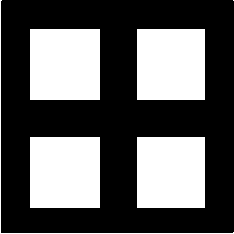
\includegraphics[width=1.0em]{CrossTile.pdf}}}}\expandafter\def\csname corpus@mysymbol@WestTile\endcsname{\raisebox{-.3em}{\mbox{
\includegraphics[width=1.0em]{WestTile.pdf}}}}\expandafter\def\csname corpus@mysymbol@NorthTile\endcsname{\raisebox{-.3em}{\mbox{
\includegraphics[width=1.0em]{NorthTile.pdf}}}}\expandafter\def\csname corpus@mysymbol@SouthTile\endcsname{\raisebox{-.3em}{\mbox{
\includegraphics[width=1.0em]{SouthTile.pdf}}}}\expandafter\def\csname corpus@mysymbol@EastTile\endcsname{\raisebox{-.3em}{\mbox{
\includegraphics[width=1.0em]{EastTile.pdf}}}}
\newcommand{\tileC}{\mysymbol{CrossTile}}       %
\newcommand{\tileW}{\mysymbol{WestTile}}      %
\newcommand{\tileN}{\mysymbol{NorthTile}}       %
\newcommand{\tileS}{\mysymbol{SouthTile}}       %
\newcommand{\tileE}{\mysymbol{EastTile}}       %
\newcommand{\tilevariable}{*}       %
\newcommand{\tiling}{TILING}
\begin{document}
\section*{1533. NEXP-completeness of fixed-rule square tiling with binary side length as the only input}
Daniel Gottesman and Sandy Irani. \emph{The Quantum and Classical Complexity of Translationally-Invariant Tiling and Hamiltonian Problems}. Theory of Computing volume 9 article 2 (2013), official complete journal PDF acquired 2026-09-30; canonical DOI 10.4086/toc.2013.v009a002 verified against official landing and printed PDF header. \url{https://theoryofcomputing.org/articles/v009a002/}. CC BY3.0.
\paragraph{Selected problem and scope (editorial).} Exact original Theorem2.2 only: fixed finite tile set, horizontal/vertical constraints and one designated tile in all four corners; the sole varying input is the positive square side length N in binary. Complete source counter/padding context, all boundary/Turing/layer-coupling rule tables and the full two-layer human proof are retained. Five original unlabeled geometric boundary-tile assets contain no digit, variable, state label, formula or proof text; every table entry, condition and Turing-machine formula is native editable TeX. Standard binary-counter Turing machines, padding and Turing tiling background remain the explicitly authored prerequisites. Periodic, weighted, reflection-symmetric and quantum variants are unselected and not counted.
\paragraph{Difficulty (editorial).} The target encodes an arbitrary nondeterministic exponential-time input into binary side length while keeping all tile rules fixed. After standard padding and counter-machine prerequisites, the authored proof still requires complete boundary forcing, opposite-direction two-layer simulation, output-to-input coupling, unique-head initialization and accepting-top enforcement at1172–1444. The full compatibility tables are retained; this fixed-rule input-encoding reduction is one H2 task beyond ordinary Cook–Levin tiling exercises.
\paragraph{Formatting (editorial).} Exact human-authored mathematical body, formulas and order retained. Only standalone front matter/typography, original counter restoration, bibliography presentation and declared noncore printed locators are adapted. Non-rendered comment prose excluded while percent newline guards remain. No mathematical argument, correction or reconstruction generated.
\clearpage
\setcounter{section}{1}
\section{Problems and results}
\label{sec:results}

The paper contains a variety of different but related results involving classical tiling and
quantum Hamiltonian problems with translational invariance.  In this section, we will
summarize the different variants, giving the proofs and more detailed discussion of
each variant in later sections.  While there are certain recurring techniques, the
details of the different cases vary considerably.

\subsection{Tiling results}

\begin{definition}{\bf \tiling}

\noindent
{\bf Problem Parameters:} A set of tiles $T = \{t_1,\ldots,t_m\}$.
A set of horizontal constraints $H \subseteq T \times T$ such that if
$t_i$ is placed to the left of $t_j$, then it must be the case that
$(t_i,t_j) \in H$. A set of vertical constraints $V \subseteq T \times T$ such that if
$t_i$ is placed below $t_j$, then it must be the case that
$(t_i,t_j) \in V$. A designated tile $t_1$ that must be placed in the four corners of the grid.


\noindent
{\bf Problem Input:} Positive integer $N$, specified in binary.



\noindent
{\bf Output:} Determine whether there is a valid tiling of an $N \times N$ grid.
\end{definition}





\begin{theorem}
\label{th:unweighted-tiling}
There exists a $(T,H,V,t_1)$ for which \tiling\ is \NEXP-complete.
\end{theorem}


A similar comment holds for all the hardness results given in this paper.
Although \expref{Theorem}{th:unweighted-tiling} is subsumed by a result proven
independently in~\cite{BGL09}, for completeness,
we give the proof in \expref{Section}{sec:tiling}. The basic idea is that the
corner tiles are used to create a border around the perimeter of the grid which
allows us to implement special rules at the top and bottom rows.
The interior of the grid is tiled in two layers.
The set of colors for the interior tiles is the cartesian product of the
layer 1 colors and the layer 2 colors.
The rules for the two layers are independent except at the boundary.
Thus, in the interior of the grid, two tiles can be placed next to each
other as long as the placement is consistent with  the layer 1 colors for
the tiles (according to the layer 1 rules) and the layer 2 colors for the tiles
(according to the later 2 rules).
In the construction, each layer implements
the action of a Turing machine.
The first TM proceeds from top to bottom
on layer 1 and the second proceeds from bottom to top on layer 2.
The first TM takes no input and acts
as a binary counter for $N$ steps. The bottom row
of  the first layer then
holds a binary number that is $\Theta(N^{1/k})$ for some constant $k$.
The rules for the lower boundary are then used
to copy the output from the binary counter to the bottom row of layer 2, which
acts as the input to a non-deterministic Turing machine which computes a \NEXP-complete
language.
The rules for the top boundary check whether
the final configuration on layer 2 is an accepting  state.
\cite{BGL09} goes about their proof somewhat differently although the end result is the
same. They look at a generalization of strings called \emph{pictures} which are essentially matrices
over a finite alphabet. \emph{Picture languages} are sets of these objects.
In particular, they study the complexity of recognizing unary picture languages
whose elements are squares.
They show that such a language corresponds to the set of tilable squares according to a finite
set of tiling rules if and only if the language defined by the binary representation
of the sizes of the squares is in $\NEXP$ time. This proof uses a binary counter similar to our
construction. In a separate proof, they show that finite tiling systems can
simulate an arbitrary Turing Machine.
It turns out that the width of the grid is not important in this
construction as long as it is an integer
at least $N$.

Note that it is important that we chose to have the input $N$ provided in binary.
If it were instead given in unary, there would only be one instance per problem size,
and the problem would be trivially in $\Pclass$/poly.  Thus, in order to prove
a meaningful hardness result, we are forced to move up the exponential hierarchy
and prove the problem is $\NEXP$-complete rather than $\NP$-complete.
\setcounter{section}{2}\setcounter{table}{1}
\section{Hardness of \tiling}
\label{sec:tiling}

We note that all of the problems
considered here are in $\NEXP$ since a valid tiling can be specified in
$2^{O(n)}$ bits and verified in time that is linear in the specification of the tiling.
For the result of the section, therefore, we focus on proving hardness.
The variants in Section~4 are also in $\NEXP$ by the same argument.

The construction will make use of a
binary counter Turing machine $M_{BC}$
which
starts with a blank semi-infinite tape. The head begins in a designated start
state in the left-most position of the tape. $M_{BC}$ will generate all
binary strings in lexicographic order. More specifically, there is a
function $f_{BC}: \mathbb{Z} \rightarrow \{0,1\}^*$ such that for some
constant $N_0$ and
every $N \ge N_0$, if $M_{BC}$ runs for $N$ steps, then the string $f_{BC}(N)$
will be written on the tape with the rest of the tape blank.
Moreover there are constants $c_1$ and $c_2$ such that
if $n$ is the length of the string $f_{BC}(N)$ and
$N \ge N_0$, then
$2^{c_1 n} \le N \le 2^{c_2 n}$.
We will also assume that for any binary string $x$, we can compute $N$
such that $f_{BC}(N) = x$ in time that is polynomial in the length of $x$.  In some of the variations of the problem we consider in
Section~4, we will need to put additional restrictions on $N$ (such as requiring $N$ to be odd), and in those cases, we still require
that we can find an $N$ with the appropriate restrictions such that $f_{BC}(N) = x$.

Using a standard padding argument, we can reduce any language in
$\NEXP$ to $\NTIME(2^{c_1 n})$. If $L$ is in $\NTIME(2^{n^k})$, the reduction
consists of padding an input $x$ so that its length is $|x|^k/c_1$~\cite{papa95}.
Thus, we will take an arbitrary non-deterministic Turing machine $M$ which accepts
an $\NEXP$-complete language $L$ in time $2^{c_1 n}$ and reduce it to \tiling.
The tiling rules and boundary conditions
will be specific to the Turing machine $M$ but will be independent
of any particular input. The reduction for \expref{Theorem}{th:unweighted-tiling}
then will take an input string $x$ and output
integer $N$ such that $f_{BC}(N-3)=x$. The tiling rules will have the property that
a string $x$ is in $L$ if and only if an $N \times N$ grid can be tiled according
to the tiling rules.
The Turing Machine $M_{BC}$ will be run for $N-3$ steps.
The $-3$ comes from the fact that the $N \times N$ grid holds two boundary rows as well
as the starting row.  This will leave the string $x$ on the final row of $M_{BC}$'s
computation.

\begin{proof}[Proof of \expref{Theorem}{th:unweighted-tiling}.]

The boundary conditions for the $N \times N$ grid will be that the four corners of the grid must have a designated tile type $\tileC$.
(We actually only need to use two corners as described in Section~4.1.)
First we will specify a set of boundary tiles and their constraints.
In addition to \tileC\,
there are four other kinds of boundary tiles: $\tileW$, $\tileN$, $\tileS$, $\tileE$.
We will call the rest of the tiles \emph{interior} tiles.
The tiling rules for the boundary tiles are summarized in \expref{Table}{table:fourcorners}.
\begin{table}
\begin{centering}
\begin{tabular}{lc|cccccc}
     &             &                \multicolumn{6}{c}{Tile on right} \\
     &             & $\tileC$ & $\tileW$ & $\tileE$ & $\tileN$ & $\tileS$ & $\tilevariable$ \\
 \hline
     & $\tileC$    &     N    &    N     &    N     &     Y    &     Y    &    N   \\
Tile & $\tileW$    &     N    &    N     &    N     &     N    &     N    &        \\
on   & $\tileE$    &     N    &    N     &    N     &     N    &     N    &    N   \\
left & $\tileN$    &     Y    &    N     &    N     &     Y    &     N    &    N   \\
     & $\tileS$    &     Y    &    N     &    N     &     N    &     Y    &    N   \\
 & $\tilevariable$ &     N    &    N     &          &     N    &     N    &        \\
\end{tabular}
\qquad
\begin{tabular}{lc|cccccc}
       &             &                \multicolumn{6}{c}{Tile on top} \\
       &             & $\tileC$ & $\tileW$ & $\tileE$ & $\tileN$ & $\tileS$ & $\tilevariable$ \\
 \hline
       & $\tileC$    &     N    &    Y     &    Y     &     N    &     N    &    N   \\
Tile   & $\tileW$    &     Y    &    Y     &    N     &     N    &     N    &    N   \\
on     & $\tileE$    &     Y    &    N     &    Y     &     N    &     N    &    N   \\
bottom & $\tileN$    &     N    &    N     &    N     &     N    &     N    &    N   \\
       & $\tileS$    &     N    &    N     &    N     &     N    &     N    &        \\
   & $\tilevariable$ &     N    &    N     &    N     &          &     N    &        \\
\end{tabular}
\caption{The tiling rules for boundary tiles.  $\tilevariable$ represents any interior tile.  ``N'' indicates a disallowed pairing of tiles.  For two boundary tiles, ``Y'' represents an allowed pairing.  Some of the rules for interior tiles are not specified, because they depend on the specific interior tile.}
\label{table:fourcorners}
\end{centering}
\end{table}

\tileW\ will mark the left side of the grid, \tileN\ the top of the
grid, \tileS\ the bottom of the grid, and \tileE\ the right side
of the grid. (See \expref{Figure}{fig:fourcorners}.)
\begin{figure}
\begin{centering}
\begin{tabular}{c@{\extracolsep{0.1em}}c@{}c@{}c@{}c}
\tileC & \tileN & \tileN & \tileN & \tileC \\
\tileW & & & & \tileE \\
\tileW & & & & \tileE \\
\tileW & & & & \tileE \\
\tileC & \tileS & \tileS & \tileS & \tileC
\end{tabular}
\caption{The only allowed tiling of the sides of a $5 \times 5$ grid.}
\label{fig:fourcorners}
\end{centering}
\end{figure}
To show that in any valid tiling the boundary tiles must be placed
in this manner, note the following facts:
\begin{itemize}
\item Nothing can go to the left of a $\tileW$ tile which means that
the only place a $\tileW$ tile could go is the left-most boundary.

\item Similarly, $\tileN$ tiles can only go in the
top row, $\tileS$ tiles can only go in the bottom row, and $\tileE$ tiles can only go in the right-most column.

\item No interior tile can border a $\tileC$ tile in any direction. Furthermore
a $\tileC$ cannot border on itself in any direction. This means that the
only possible locations for a $\tileC$ are the four corners since those
are the only places which can be surrounded by $\tileW$, $\tileN$, $\tileS$, or $\tileE$
tiles. Since the boundary conditions state that $\tileC$ tiles must go in
the corners, those are exactly the locations that will hold $\tileC$
tiles.

\item The only tiles that can go above or below a $\tileC$ tile are $\tileW$ and $\tileE$ tiles, and
$\tileE$ cannot go on the west boundary.  Thus, the tiles on the west boundary adjacent to the corners
must be $\tileW$ tiles.

\item Only $\tileW$ or $\tileC$ can go above or below a $\tileW$ tile, so the entire west boundary, except for the corners, will be $\tileW$ tiles.

\item Similar logic shows that the entire east boundary, except for the corners, will be $\tileE$ tiles.  Also, the entire south boundary, except for the corners, will be $\tileS$ tiles, and the entire north boundary, except for the corners, will be $\tileN$ tiles.

\end{itemize}

The remainder of the grid will be tiled in two layers.
The constraints on the two layers only interact at the bottom of the grid, so
we describe each layer separately. The actual type for an
interior tile is specified by a pair denoting its
layer 1 type and layer 2 type.
The bottom layer will be used to simulate the Turing machine $M_{BC}$.
The top boundary of the grid will be used to ensure that $M_{BC}$
begins with the proper initial conditions. Then the rules will enforce that
each row of the tiling going downwards advances the Turing machine $M_{BC}$
by one step. At the bottom of the grid, the output is copied onto layer 2.
Layer 2 is then used to simulate a generic non-deterministic Turing machine
on the input copied from layer 1. The lower left corner is used to
initialize the state of $M$ and the constraints enforce that
each row going upwards advances the Turing machine $M$ by one step.
Finally, the only states of $M$ that are allowed to be below an $\tileN$ tile
are accepting states.
Since each Turing machine only executes for $N-3$ steps and the grid has space
for $N-2$ tape symbols, the right end of the tape will never be reached.



Although it is well known that tiling rules are Turing complete~\cite{kmw62},
we review the ideas here in order to specify the details in our
construction. We will assume that the Turing machine $M$ is encoded
in a tiling that goes from bottom to top. This can easily be reversed for
$M_{BC}$ which goes from top to bottom.
The non-deterministic Turing machine $M$ is specified by
a triplet $(\Sigma, Q, \delta)$, with
designated blank symbol $\# \in \Sigma$, start state $q_0 \in Q$ and
accept state $q_A \in Q$.
There are three varieties of tiles, designated by elements of
$\Sigma$ (variety 1), $\Sigma \times Q \times \{r,l\}$ (variety 2) and
$\Sigma \times Q \times \{R,L\}$ (variety 3).  Variety 1 represents the state of the tape away from the Turing machine head.  Variety 2 represents the
state of the tape and head when the head has moved on to a location but before it has acted.  The $\{r, l\}$ symbol in a variety 2 tile tells us from which direction the head came in its last move.  Variety 3 represents the state of the tape and head after
the head has acted, and the $\{R,L\}$ symbol tells us which way the head moved.

The tiling rules are given in \expref{Table}{table:TM}.
%
\begin{table}
\begin{centering}
\begin{tabular}{lc|cccccc}
     &             &                \multicolumn{6}{c}{Tile on right} \\
     &             & $[b]$ & $[b,q',r]$ & $[b,q',l]$ & $[b,q',R]$ & $[b,q',L]$ & $\tileE$ \\
 \hline
     & $[a]$       &   Y   &     Y      &      N     &      Y     &     N      &   Y     \\
Tile & $[a,q,r]$   &   N   &     N      &      N     &      N     & If $q=q'$  &   N     \\
on   & $[a,q,l]$   &   Y   &     N      &      N     &      N     &     N      &   Y     \\
left & $[a,q,R]$   &   N   &     N      & If $q=q'$  &      N     &     N      &   N     \\
     & $[a,q,L]$   &   Y   &     N      &      N     &      N     &     N      &   Y     \\
     & $\tileW$    &   Y*  &     Y     & If $q'=q_0$ &      Y     &     N      &   Y     \\
\end{tabular}

\bigskip
\begin{tabular}{lc|ccccc}
       &             &                \multicolumn{5}{c}{Tile on top} \\
       &             & $[b]$    & $[b,q',r]$ & $[b,q',l]$                & $[b,q',R]$ & $[b,q',L]$ \\
 \hline
       & $[a]$       & If $a=b$ &  If $a=b$  &  If $a=b$, $q' \neq q_0$  &     N      &     N   \\
Tile   & $[a,q,r]$   &    N     &     N      &     N                     & If TM rule & If TM rule \\
on     & $[a,q,l]$   &    N     &     N      &     N                     & If TM rule & If TM rule \\
bottom & $[a,q,R]$   & If $a=b$ &  If $a=b$  &  If $a=b$, $q' \neq q_0$  &     N      &     N   \\
       & $[a,q,L]$   & If $a=b$ &  If $a=b$  &  If $a=b$, $q' \neq q_0$  &     N      &     N   \\
\end{tabular}
\caption{The tiling rules to simulate a Turing machine.  ``N'' indicates a disallowed pairing of tiles, and ``Y'' represents an allowed pairing.  Pairings with ``if'' statements are allowed only if the condition is satisfied.  ``If TM rule'' means the pairing is allowed only if $(a,q) \rightarrow (b,q',L/R)$ is one of the valid non-deterministic moves of the Turing machine being simulated.  The ``Y*'' entry will be modified later to get the correct starting configuration for the Turing machine. }
\label{table:TM}
\end{centering}
\end{table}
%
%
The table below gives an example of a section of tiles that
encodes the move $(a,q) \rightarrow (b,q',L)$ of the Turing machine from the bottom
row to the middle row and the move $(c,q') \rightarrow (f,q'',R)$ from
the middle row to the top row:

\[
\begin{array}{|c|c|c|}
\hline
[f,q'',R] & [b,q'',l] & [d] \\
\hline
[c,q',r] & [b,q',L] & [d] \\
\hline
[c] & [a,q,r] & [d,q,L]\\
\hline
\end{array}
\]

The lower row shows the head in the square with the $a$. The $[d,q,L]$
is from the previous TM move.
The tile $[b,q',L]$ in the middle row
enforces that the tiler is committing to executing the
step $(a,q) \rightarrow (b,q',L)$, although there may have been
other possible non-deterministic choices. The $[c,q',r]$ tile to the left of
the $[b,q',L]$ shows the new location and state of the head after the first move.
The $[b,q',L]$ tile now just acts as a $[b]$ tile for purposes of
the tiling above. The tile $[f,q'',R]$ enforces that the
tiler is committing to executing the step $(c,q') \rightarrow (f,q'',R)$.
The $[b,q'',l]$ tile to the right of
the $[f,q'',R]$ shows the new location and state of the head after the second move.


To be consistent with the horizontal tiling rules, a row must consist of some number of variety 1 tiles, along with adjacent pairs consisting of a variety 2 tile and a variety 3 tile.  The variety 2 and 3 tiles must be matched in the following sense: $q = q'$, and either we have $r$ on the left and $L$ on the right or $R$ on the left and $l$ on the right.
%
At the west edges of the row, we could possibly have just a single variety 2 tile by itself.
However, this can only happen if the tile is of the form $[a,q,l]$.
The rules enforce then that a \tileW\ tile can only go to the left of a variety 2 tile if
the Turing Machine state is $q_0$, which
is the starting head state of the machine.  We can assume without loss of
generality that the Turing machine never transitions back to the $q_0$ state, and
never has a transition that would move it left from the first location on the tape.
%
Given that we have one row of this form, the next row up must have the
same number of pairs of variety 2 and variety 3 tiles, and furthermore,
each pair must be shifted one position left or right, with the Turing
machine performing an allowed transition, as in the example.  If one row
has exactly one variety 2 tile $[a,q_0,l]$ in the leftmost position, then every row
above it in a valid tiling will also have exactly one variety 2 tile, and the $j$th
row up will correctly represent the state of the Turing machine tape and head after $j$ steps.

For our particular tiling, we will need additional rules for some pairs of boundary tiles and interior tiles.  These additional rules will be different for layers $1$ and $2$, and some of them will couple the two layers.  In addition, we will need to slightly modify some of the horizontal tiling rules.  The new and modified rules are summarized in \expref{Table}{table:TMboundaries}.  Also, for layer $1$, recall that we reverse ``above'' and ``below'' for the regular Turing machine simulation rules (\expref{Table}{table:TM}), so that time goes downwards instead of upwards.
\begin{table}
Additional layer $1$ rules:
\smallskip
\begin{centering}
\begin{tabular}{lc|ccccc}
\multicolumn{2}{l|}{Boundary Tile} &                \multicolumn{5}{c}{Adjacent interior tile} \\
\multicolumn{2}{l|}{Location} & $[a]$ & $[a,q,r]$ & $[a,q,l]$          & $[a,q,R]$ & $[a,q,L]$ \\
 \hline
Bottom & $\tileS$    &    Y        &     Y     &         Y             &    Y      &    Y     \\
Top    & $\tileN$    & If $a=\#$   &     N     & If $a=\#$ and $q=q_0$ &    N      &    N      \\
Left   & $\tileW$    & If $a \neq \#$ &  Y     & If $q=q_0$            &    Y      &    N      \\
\end{tabular}

\bigskip

\end{centering}
\noindent Additional layer $2$ rules:
\smallskip
\begin{centering}
\begin{tabular}{lc|ccccc}

\multicolumn{2}{l|}{Boundary Tile} &                \multicolumn{5}{c}{Adjacent interior tile} \\
\multicolumn{2}{l|}{Location} & $[a]$         & $[a,q,r]$  & $[a,q,l]$                            & $[a,q,R]$ & $[a,q,L]$ \\
 \hline
Bottom  & $\tileS$ & If $a$ matches layer $1$ &     N
& \parbox{30mm}{\centering If $q=q_0$ and\\ $a$ matches layer $1$} &    N      &    N      \\
Top     & $\tileN$ &   Y                      & If $q=q_A$ & If $q=q_A$                           &    Y      &    Y      \\
Left    & $\tileW$ & If $a \not\in \Sigma_{M_{BC}}$ &  Y   & If $q=q_0$                           &    Y      &    N      \\
\end{tabular}

\caption{Additional tiling rules between certain boundary and interior tiles for
layers $1$ and $2$.  Note that these rules are specific to the boundary
only because we have established that the boundary tiles can only
be placed at the boundary.
For layer $2$, the alphabet symbol $a \in \Sigma$ must match the alphabet symbol for the corresponding layer $1$ tile when on the bottom interior row.}
\label{table:TMboundaries}
\end{centering}
\end{table}

We would like to start out the
Turing machine $M_{BC}$ with $[\#, q_0, l]$ in the leftmost location
followed by $[\#]$ tiles.  This is ensured by the additional rules for layer $1$: The top interior row must consist of only these two types of tiles, and the leftmost location cannot be $[\#]$.  Since there cannot be any variety 3 tiles, there can only be one $[\#, q_0, l]$ in the leftmost location.
We can assume without loss of generality that
the Turing machine overwrites the leftmost $\#$ on the tape
and never writes a $\#$ there again.

The rest of the layer 1 rules just enforce the rules for the Turing machine
$M_{BC}$.

Now in order to copy the output from $M_{BC}$ to the input tape
for $M$, we restrict the kinds of tiles that can go above $\tileS$ tiles.
All the alphabet characters in the bottom interior row of layer 2 must
match the alphabet characters for layer 1.  That is, the output of $M_{BC}$ is
copied onto the input of $M$.

We also want to ensure that the starting configuration of $M$ has
only one head in the leftmost location.  To accomplish this,
we forbid a $\tileW$ to go next to an $[a]$ tile for $a \in \Sigma_{M_{BC}}$, so
the leftmost tile in the 2nd row from the bottom of layer 2 must be $[a,q_0,l]$.  Since there
can be no variety 3 tiles in the 2nd row, that must be the only variety 2 tile
in the row.  A little care must be taken to overwrite the leftmost input tape
character with something that is not in the alphabet of $M_{BC}$.
This is because we have forbidden having an $[a]$ tile to the right
of a $\tileW$ for any $a \in \Sigma_{M_{BC}}$, and this prohibition
applies to \emph{all} rows.
The information encoded in the left-most tape symbol can be retained by
having a new $a'$ symbol in $\Sigma_M$ for every $a \in \Sigma_{M_{BC}}$.

Finally, the only variety 2 tiles on layer 2 which we allow below a
$\tileN$ tile must be of the form $[a,q_A, r/l]$, where $q_A$ is the accepting state.
Thus, there is a valid tiling if and only if the non-deterministic TM $M$ accepts on input $x$ in $N-3$ steps.
\end{proof}
\clearpage
\begingroup\raggedright
%
%
%
%
%
\providecommand{\bibhead}[1]{}
%
\expandafter\ifx\csname pdfbookmark\endcsname\relax%
  \providecommand{\tocrefpdfbookmark}{}
\else\providecommand{\tocrefpdfbookmark}{%
   \hypertarget{tocreferences}{}%
   \pdfbookmark[1]{References}{tocreferences}}%
\fi

\tocrefpdfbookmark
\begin{thebibliography}{10}

\bibitem{focsVersion}\bibhead{focsVersion}
{\sc Dorit Aharonov, Daniel Gottesman, Sandy Irani, and Julia Kempe}: The power
  of quantum systems on a line.
\newblock In {\em Proc. 48th FOCS}, pp. 373--383. IEEE Comp. Soc. Press, 2007.
\newblock [\epfmtdoi{10.1109/FOCS.2007.46}]

\bibitem{QMA1D}\bibhead{QMA1D}
{\sc Dorit Aharonov, Daniel Gottesman, Sandy Irani, and Julia Kempe}: The power
  of quantum systems on a line.
\newblock {\em Comm. Math. Physics}, 287(1):41--65, 2009.
\newblock Preliminary version at \href{http://arxiv.org/abs/0705.4077}{arXiv}.
  Extended abstract in \href{http://dx.doi.org/10.1109/FOCS.2007.46}{FOCS'07}.
\newblock [\epfmtdoi{10.1007/s00220-008-0710-3}]

\bibitem{bcg89}\bibhead{bcg89}
{\sc Shai Ben-David, Benny Chor, Oded Goldreich, and Michael Luby}: On the
  theory of average case complexity.
\newblock {\em J. Comput. System Sci.}, 44(2):193--219, 1992.
\newblock Preliminary version in
  \href{http://dx.doi.org/10.1145/73007.73027}{STOC'89}.
\newblock [\epfmtdoi{10.1016/0022-0000(92)90019-F}]

\bibitem{berger66}\bibhead{berger66}
{\sc Robert Berger}: The undecidability of the domino problem.
\newblock {\em Memoirs of the Am. Math. Soc.}, 66:1--72, 1966.

\bibitem{bernsteinVazirani}\bibhead{bernsteinVazirani}
{\sc Ethan Bernstein and Umesh Vazirani}: Quantum complexity theory.
\newblock {\em SIAM J. Comput.}, 26(5):1411--1473, 1997.
\newblock Preliminary version in
  \href{http://dx.doi.org/10.1145/167088.167097}{STOC'93}.
\newblock [\epfmtdoi{10.1137/S0097539796300921}]

\bibitem{BGL09}\bibhead{BGL09}
{\sc Alberto Bertoni, Massimiliano Goldwurm, and Violetta Lonati}: The
  complexity of unary tiling recognizable picture languages: Nondeterministic
  and unambiguous cases.
\newblock {\em Fundam. Inform.}, 91(2):231--249, 2009.
\newblock Preliminary version in
  \href{http://dx.doi.org/10.1007/978-3-540-70918-3_33}{STACS'07}.
\newblock [\epfmtdoi{10.3233/FI-2009-0042}]

\bibitem{BM94}\bibhead{BM94}
{\sc Jean-Philippe Bouchaud and Marc M{\'e}zard}: Self induced quenched
  disorder: A model for the glass transition.
\newblock {\em J. Phys. I France}, 4(8):1109--1114, 1994.
\newblock Preprint at \href{http://arxiv.org/abs/cond-mat/9405075}{arXiv}.
\newblock [\epfmtdoi{10.1051/jp1:1994240}]

\bibitem{deutsch}\bibhead{deutsch}
{\sc David {Deutsch}}: {Quantum theory, the Church-Turing principle and the
  universal quantum computer}.
\newblock {\em Proc. Royal Society of London Series A}, 400(1818):97--117,
  1985.
\newblock [\epfmtdoi{10.1098/rspa.1985.0070}]

\bibitem{boas97}\bibhead{boas97}
{\sc Peter~van Emde~Boas}: The convenience of tilings.
\newblock In {\sc Andrea Sorbi}, editor, {\em Complexity, Logic, and Recursion
  Theory}, pp. 331--363. Marcel Dekker Inc, 1997.

\bibitem{Furer83}\bibhead{Furer83}
{\sc Martin F{\"u}rer}: The computational complexity of the unconstrained
  limited domino problem (with implications for logical decision problems).
\newblock In {\em Logic and Machines: Decision and Complexity}, volume 171 of
  {\em LNCS}, pp. 312--319. Springer, 1984.
\newblock [\epfmtdoi{10.1007/3-540-13331-3\_48}]

\bibitem{GW83}\bibhead{GW83}
{\sc Hana Galperin and Avi Wigderson}: Succinct representations of graphs.
\newblock {\em Inf. Control}, 56(3):183--198, 1983.
\newblock [\epfmtdoi{10.1016/S0019-9958(83)80004-7}]

\bibitem{arxiv-version}\bibhead{arxiv-version}
{\sc Daniel Gottesman and Sandy Irani}: The quantum and classical complexity of
  translationally invariant tiling and {H}amiltonian problems, 2009.
\newblock Conference version in
  \href{http://dx.doi.org/10.1109/FOCS.2009.22}{FOCS'09}.
\newblock [\epfmt{arxiv}{0905.2419}]

\bibitem{gradel89}\bibhead{gradel89}
{\sc Erich Gr{\"a}del}: Dominoes and the complexity of subclasses of logical
  theories.
\newblock {\em Ann. Pure Appl. Logic}, 43(1):1--30, 1989.
\newblock [\epfmtdoi{10.1016/0168-0072(89)90023-7}]

\bibitem{ingham}\bibhead{ingham}
{\sc Albert~E. Ingham}: On the difference between consecutive primes.
\newblock {\em Quarterly Journal of Mathematics (Oxford Series)},
  8(1):255--266, 1937.
\newblock [\epfmtdoi{10.1093/qmath/os-8.1.255}]

\bibitem{irani09}\bibhead{irani09}
{\sc Sandy Irani}: Ground state entanglement in one dimensional translationally
  invariant quantum systems.
\newblock {\em J. Math. Phys.}, 51(2):022101, 2010.
\newblock Preprint at \href{http://arxiv.org/abs/0901.1107}{arXiv}.
\newblock [\epfmtdoi{10.1063/1.3254321}]

\bibitem{JWZtranslation}\bibhead{JWZtranslation}
{\sc Dominik Janzing, Pawel Wocjan, and Shengyu Zhang}: A single-shot
  measurement of the energy of product states in a translation invariant spin
  chain can replace any quantum computation.
\newblock {\em New J. Phys.}, 10(9):093004, 2008.
\newblock Preprint at \href{http://arxiv.org/abs/0710.1615}{arXiv}.
\newblock [\epfmtdoi{10.1088/1367-2630/10/9/093004}]

\bibitem{JV09}\bibhead{JV09}
{\sc Emmanuel Jeandel and Pascal Vanier}: Periodicity in tilings.
\newblock In {\em 14th Internat. Conf. Developments in Language Theory
  (DLT'10)}, pp. 243--254. Springer, 2010.
\newblock Preprint at \href{http://arxiv.org/abs/0909.3997}{arXiv}.
\newblock [\epfmtdoi{10.1007/978-3-642-14455-4\_23}]

\bibitem{JS74}\bibhead{JS74}
{\sc Neil~D. Jones and Alan~L. Selman}: Turing machines and the spectra of
  first-order formulas.
\newblock {\em J. Symbolic Logic}, 39(1):139--150, 1974.
\newblock Available at \href{http://www.jstor.org/stable/2272354}{JSTOR}.
  Preliminary version in
  \href{http://dx.doi.org/10.1145/800152.804909}{STOC'72}.

\bibitem{kmw62}\bibhead{kmw62}
{\sc A.~S. Kahr, Edward~F. Moore, and Hao Wang}: Entscheidungsproblem reduced
  to the {$\forall \exists \forall$} case.
\newblock {\em Proc. Natl. Acad. Sci. USA}, 48(3):365--377, 1962.
\newblock \href{http://www.jstor.org/stable/71207}{JSTOR}.

\bibitem{Kaytranslation}\bibhead{Kaytranslation}
{\sc Alastair Kay}: Computational power of symmetric {H}amiltonians.
\newblock {\em Phys. Rev. A}, 78(1):012346, 2008.
\newblock Preprint at \href{http://arxiv.org/abs/0801.3228}{arXiv}.
\newblock [\epfmtdoi{10.1103/PhysRevA.78.012346}]

\bibitem{KempeKitaevRegev06}\bibhead{KempeKitaevRegev06}
{\sc Julia Kempe, Alexei Kitaev, and Oded Regev}: The complexity of the local
  {H}amiltonian problem.
\newblock {\em SIAM J. Comput.}, 35(5):1070--1097, 2006.
\newblock Preliminary version in
  \href{http://dx.doi.org/10.1007/978-3-540-30538-5_31}{FSTTCS'04}.
\newblock [\epfmtdoi{10.1137/S0097539704445226}]

\bibitem{Kitaev:book}\bibhead{Kitaev:book}
{\sc Alexei Kitaev, Alexander~H. Shen, and Michael~N. Vyalyi}: {\em Classical
  and Quantum Computation}.
\newblock AMS, 2002.
\newblock [\epfmt{acm}{863284}]

\bibitem{levin86}\bibhead{levin86}
{\sc Leonid~A. Levin}: Average case complete problems.
\newblock {\em SIAM J. Comput.}, 15(1):285--286, 1986.
\newblock Preliminary version in
  \href{http://dx.doi.org/10.1145/800057.808713}{STOC'84}.
\newblock [\epfmtdoi{10.1137/0215020}]

\bibitem{lewis78}\bibhead{lewis78}
{\sc Harry~R. Lewis}: Complexity of solvable cases of the decision problem for
  the predicate calculus.
\newblock In {\em Proc. 19th FOCS}, pp. 35--47. IEEE Comp. Soc. Press, 1978.
\newblock [\epfmtdoi{10.1109/SFCS.1978.9}]

\bibitem{lp97}\bibhead{lp97}
{\sc Harry~R. Lewis and Christos~H. Papadimitriou}: {\em Elements of the Theory
  of Computation}.
\newblock Prentice Hall, 2 edition, 1997.
\newblock [\epfmt{acm}{549820}]

\bibitem{LCV}\bibhead{LCV}
{\sc Yi-Kai Liu, Matthias Christandl, and Frank Verstraete}: Quantum
  computational complexity of the {$N$}-representability problem: {Q}{M}{A}
  complete.
\newblock {\em Phys. Rev. Lett.}, 98(11):110503, 2007.
\newblock Preprint at \href{http://arxiv.org/abs/quant-ph/0609125}{arXiv}.
\newblock [\epfmtdoi{10.1103/PhysRevLett.98.110503}]

\bibitem{NWtranslation}\bibhead{NWtranslation}
{\sc Daniel Nagaj and Pawel Wocjan}: Hamiltonian quantum cellular automata in
  one dimension.
\newblock {\em Phys. Rev. A}, 78(3):032311, 2008.
\newblock Preprint at \href{http://arxiv.org/abs/0802.0886}{arXiv}.
\newblock [\epfmtdoi{10.1103/PhysRevA.78.032311}]

\bibitem{Oliveira:05a}\bibhead{Oliveira:05a}
{\sc Roberto Oliveira and Barbara~M. Terhal}: The complexity of quantum spin
  systems on a two-dimensional square lattice.
\newblock {\em Quantum Information {\&} Computation}, 8(10):900--924, 2008.
\newblock Preprint at \href{http://arxiv.org/abs/quant-ph/0504050}{arXiv}.
\newblock [\epfmt{acm}{2016987}]

\bibitem{papa95}\bibhead{papa95}
{\sc Christos~H. Papadimitriou}: {\em Computational Complexity}.
\newblock Addison-Wesley, 1995.

\bibitem{PY86}\bibhead{PY86}
{\sc Christos~H. Papadimitriou and Mihalis Yannakakis}: A note on succinct
  representations of graphs.
\newblock {\em Inf. Control}, 71(3):181--185, 1986.
\newblock [\epfmtdoi{10.1016/S0019-9958(86)80009-2}]

\bibitem{P66}\bibhead{P66}
{\sc Rohit Parikh}: On context-free languages.
\newblock {\em J. ACM}, 13(4):570--581, 1966.
\newblock [\epfmtdoi{10.1145/321356.321364}]

\bibitem{RothWin00}\bibhead{RothWin00}
{\sc Paul W.~K. Rothemund and Erik Winfree}: The program-size complexity of
  self-assembled squares.
\newblock In {\em Proc. 32nd STOC}, pp. 459--468. ACM Press, 2000.
\newblock [\epfmtdoi{10.1145/335305.335358}]

\bibitem{valiant79}\bibhead{valiant79}
{\sc Leslie~G. Valiant}: The complexity of enumeration and reliability
  problems.
\newblock {\em SIAM J. Comput.}, 8(3):410--421, 1979.
\newblock [\epfmtdoi{10.1137/0208032}]

\bibitem{wang61}\bibhead{wang61}
{\sc Hao Wang}: Proving theorems by pattern recognition {II}.
\newblock {\em Bell Systems Technical Journal}, 40:1--41, 1961.

\bibitem{Win98}\bibhead{Win98}
{\sc Erik Winfree}: {\em Algorithmic Self-Assembly of DNA}.
\newblock Ph.\,D.\ thesis, California Institute of Technology, 1998.

\end{thebibliography}
\endgroup
\end{document}
